\chapter{Analyse des résultats}

% % \index{résultats}
% À ce stade, vous avez mené à bien votre projet, réalisé vos expériences, collecté vos données et procédé à leur analyse. Il est désormais temps de présenter vos résultats et d'en proposer une interprétation approfondie. Cette étape est déterminante pour valider la pertinence et la rigueur de votre travail.

% % \index{objectifs}
% Vous devez démontrer que vos objectifs ont été atteints, que vous avez répondu aux questions de recherche initiales et que vous avez apporté une solution pertinente au problème posé. Il s'agit ici de convaincre le lecteur de la valeur scientifique ou technique de vos résultats.

% Prenez soin de ne pas submerger votre rapport d'une quantité excessive de données brutes qui n'apporteraient pas de valeur ajoutée à votre analyse. Il est naturel, après un travail rigoureux, d'avoir accumulé un grand volume de données. Privilégiez celles qui contribuent à démontrer vos conclusions et à appuyer votre argumentation.
\newpage
\section{Présentation des résultats}\label{ResultsShow}
Une fois l'application téléchargée sur téléphone. On peut pointer la caméra du smartphone vers le
petit bâtiment qu'on reconnaît de l'éditeur Unity (cf. \ref{AddObject}) et le cube apparaît.

Un autre point important auquel il faut faire attention sont les anchors qu'on peut générer en cliquant sur l'écran, elles sont au
nombre de quatre sur la figure \ref{fig:GeoSample} et sont visibles sur la route. C'est grâce à cette méthode (le \acrshort{raycast})
qu'on va pouvoir interagir avec les objets virtuels.

\begin{figure}[H]
    \centering
    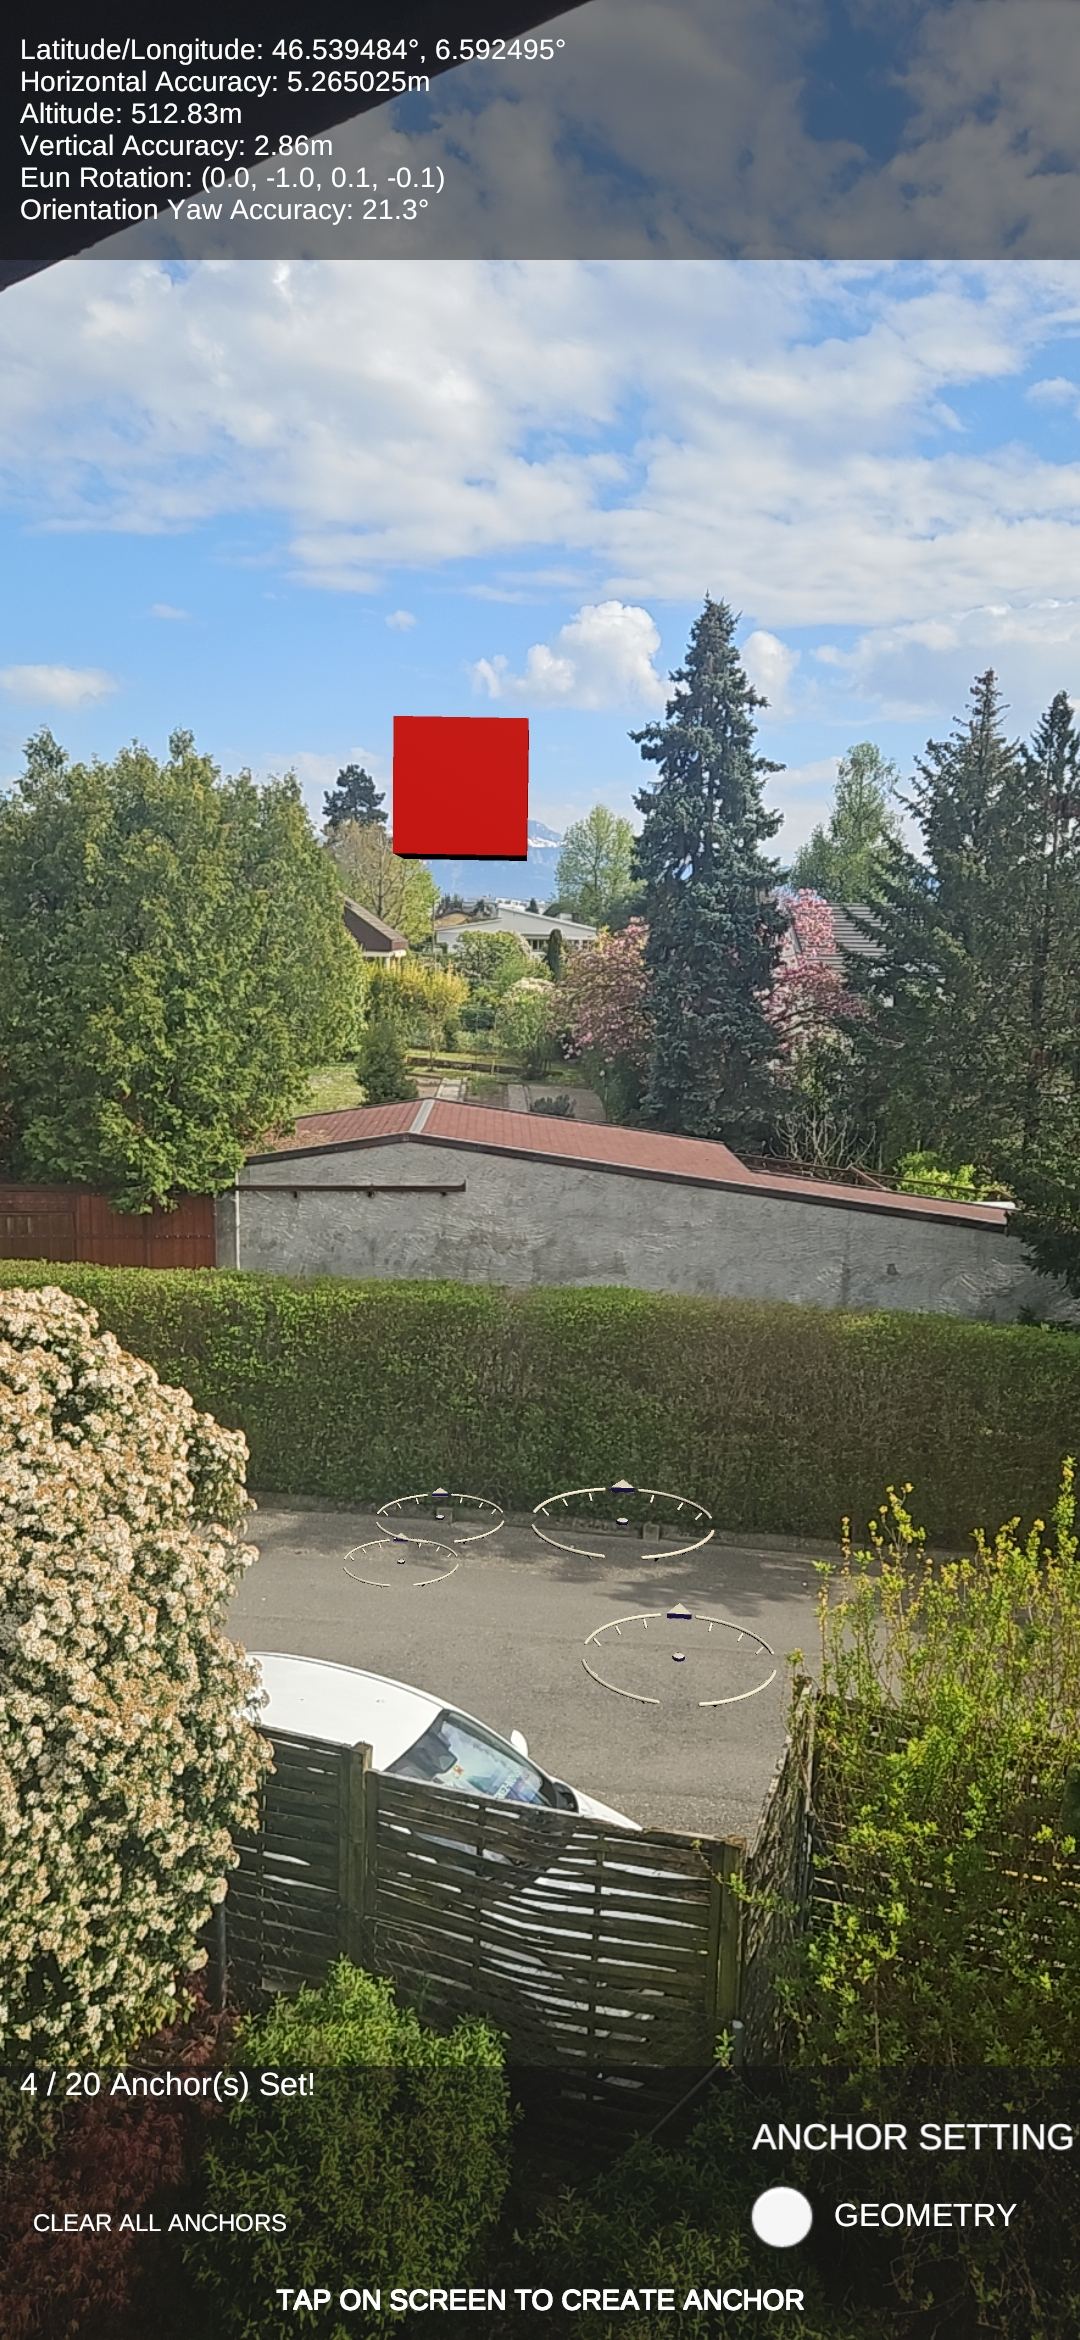
\includegraphics[width=0.5\linewidth]{assets/figures/Screenshots/geospatial example.jpg}
    \caption{Vue de l'objet virtuel ajouté depuis le smartphone.}
    \label{fig:GeoSample}
\end{figure}
% La présentation des résultats doit être claire et synthétique. Commencez par exposer les données essentielles de manière structurée, en utilisant des supports visuels pertinents tels que des tableaux, des graphiques, des schémas, des figures, des photographies ou des extraits de code. Ces éléments doivent être soigneusement légendés et accompagnés de commentaires explicatifs.

% Chaque résultat présenté doit être brièvement interprété afin d'en souligner la signification. Il ne s'agit pas seulement de montrer les données, mais d'expliquer ce qu'elles révèlent par rapport aux objectifs fixés.

% Pensez également à mentionner les unités de mesure, à signaler les éventuels biais susceptibles d'avoir influencé vos résultats et à évaluer les incertitudes associées à vos mesures ou à vos méthodes. Ces éléments sont essentiels pour garantir la rigueur scientifique de votre analyse.
\newpage
\section{Discussion des résultats}
L'application a une taille de 194 Mo à l'écriture du rapport, pour comparaison, \textit{Pikmin Bloom}, un jeu vidéo basé sur la géolocalisation qui a un mode photo AR, a une taille de 1.6 Go.
de. Bien qu'il n'y ait pas de compteur d'images par seconde pour attester de cela, les images par secondes sont constantes et aucun ralentissement n'est perceptible.
La capture d'écran de la section \ref{ResultsShow} montre différentes variables soit : la latitude et la longitude, l'altitude ainsi que la précision de ces mesures.
La mesure Eun Rotation correspond à des coordonnées "East-Up-North" où la première coordonnée (x) pointe vers l'Est, la deuxième (y) pointe vers le haut, contre la gravité et le dernier (z) pointe vers le Nord. Un article wikipedia explique ces coordonnées (appelé ENU dans l'article)\cite{LocalTangentPlane2025}.
La quatrième variable dans Eun Rotation est encore inconnue de l'étudiant. La rotation a aussi une précision donnée dans Orientation Yaw Accuracy.
% La discussion constitue une étape essentielle, car elle vous permet de donner du sens à vos résultats. Vous devez aller au-delà de la simple présentation des données en les analysant de manière critique et en les confrontant aux travaux existants.

% Cette section doit permettre :
% \begin{itemize}
%     \item De comparer vos résultats à ceux issus de la littérature ou d'études antérieures, afin de mettre en perspective vos observations.
%     \item D'évaluer la pertinence de vos résultats et d'en discuter les implications théoriques ou pratiques.
%     \item De justifier les résultats obtenus, en expliquant les causes potentielles des écarts observés ou des résultats inattendus.
%     \item D'identifier les limites de votre étude et d'en proposer des pistes d'amélioration pour de futurs travaux.
% \end{itemize}

% Cette réflexion critique démontre votre capacité à analyser vos résultats de manière approfondie et à en tirer des enseignements pertinents. Elle est essentielle pour montrer que vous maîtrisez non seulement vos données, mais également les implications qu'elles soulèvent dans le cadre de votre recherche.
